\documentclass[a4paper, 11pt]{article}

\usepackage[utf8]{inputenc}
\usepackage[T1]{fontenc}
\usepackage{graphicx, wrapfig}
\usepackage[top=3cm, bottom=3cm, left=3.2cm, right=3.2cm]{geometry}
\usepackage{lmodern}
\usepackage{fancyhdr}
\usepackage{color, colortbl}
\usepackage[usenames, dvipsnames]{xcolor}
\usepackage{amsmath}
\usepackage{amssymb}
\usepackage{mathrsfs}
\usepackage{amsthm}
\usepackage{pgf, pgfplots, tikz}
\usepackage{listings}
\usepackage{makeidx}
\usepackage{hyperref}
\usepackage{setspace}
\usetikzlibrary{calc}
\usetikzlibrary{plotmarks}
\usetikzlibrary{decorations.markings}
\usepackage{manfnt, multicol}
\usepackage[section]{algorithm}
\usepackage{algorithmicx, algpseudocode, listings}
% fixes a bug for closing parantheses
\usepackage{etoolbox}
\makeatletter
\patchcmd{\lsthk@SelectCharTable}{%
  \lst@ifbreaklines\lst@Def{`)}{\lst@breakProcessOther)}\fi}{}{}{}
\makeatother
\usepackage{array, multirow, longtable}
\usepackage{enumerate}
\usepackage[inline]{enumitem}
\usepackage[english]{babel}
\usepackage{caption, tabu}


%°°°°°°°°°°°°°°°°°°°°°°°°°°°°°°°°°°°°°°°°°°°°°°%
%----Définition de l'environnement listings----%
%°°°°°°°°°°°°°°°°°°°°°°°°°°°°°°°°°°°°°°°°°°°°°°%

\lstset{literate=
  {á}{{\'a}}1 {é}{{\'e}}1 {í}{{\'i}}1 {ó}{{\'o}}1 {ú}{{\'u}}1
  {Á}{{\'A}}1 {É}{{\'E}}1 {Í}{{\'I}}1 {Ó}{{\'O}}1 {Ú}{{\'U}}1
  {à}{{\`a}}1 {è}{{\`e}}1 {ì}{{\`i}}1 {ò}{{\`o}}1 {ù}{{\`u}}1
  {À}{{\`A}}1 {È}{{\'E}}1 {Ì}{{\`I}}1 {Ò}{{\`O}}1 {Ù}{{\`U}}1
  {ä}{{\"a}}1 {ë}{{\"e}}1 {ï}{{\"i}}1 {ö}{{\"o}}1 {ü}{{\"u}}1
  {Ä}{{\"A}}1 {Ë}{{\"E}}1 {Ï}{{\"I}}1 {Ö}{{\"O}}1 {Ü}{{\"U}}1
  {â}{{\^a}}1 {ê}{{\^e}}1 {î}{{\^i}}1 {ô}{{\^o}}1 {û}{{\^u}}1
  {Â}{{\^A}}1 {Ê}{{\^E}}1 {Î}{{\^I}}1 {Ô}{{\^O}}1 {Û}{{\^U}}1
  {œ}{{\oe}}1 {Œ}{{\OE}}1 {æ}{{\ae}}1 {Æ}{{\AE}}1 {ß}{{\ss}}1
  {ç}{{\c c}}1 {Ç}{{\c C}}1 {ø}{{\o}}1 {å}{{\r a}}1 {Å}{{\r A}}1
  {€}{{\EUR}}1 {£}{{\pounds}}1
}

\lstdefinestyle{luaCode}{
  basicstyle=\footnotesize,        	% the size of the fonts that are used for the code
  breakatwhitespace=true,         	% sets if automatic breaks should only happen at whitespace
  breaklines=true,                 	% sets automatic line breaking
  captionpos=t,                    	% sets the caption-position to bottom
  commentstyle=\footnotesize\ttfamily\color{Emerald},    	% comment style
  deletekeywords={...},            	% if you want to delete keywords from the given language
  escapeinside={¦}{¦)},         	% if you want to add LaTeX within your code
  extendedchars=true,              	% lets you use non-ASCII characters; for 8-bits encodings only, does not work with UTF-8
  rulecolor=\color{OliveGreen!80},
  frame=trbl,
  framexleftmargin=10.8pt,
  framexrightmargin=7.2pt,
  keepspaces=true,                 	% keeps spaces in text, useful for keeping indentation of code (possibly needs columns=flexible)
  keywordstyle=\small\bfseries\color{OliveGreen!80},   % keyword style
  language=[5.0]Lua,                 	% the language of the code
  morekeywords={job.position},            	% if you want to add more keywords to the set
  numbers=left,                    	% where to put the line-numbers; possible values are (none, left, right)
  numbersep=3pt,                   	% how far the line-numbers are from the code
  numberstyle=\tiny\color{Gray}, 	% the style that is used for the line-numbers
  resetmargins=false                    % sets margins to 0 in a list
  showspaces=false,                	% show spaces everywhere adding particular underscores; it overrides 'showstringspaces'
  showstringspaces=false,          	% underline spaces within strings only
  showtabs=false,                  	% show tabs within strings adding particular underscores
  stepnumber=2,                    	% the step between two line-numbers. If it's 1, each line will be numbered
  stringstyle=\color{RawSienna},     	% string literal style
  tabsize=2,                       	% sets default tabsize to 2 spaces
  title=\lstname,                   	% show the filename of files included with \lstinputlisting; also try caption instead of title
  xleftmargin=1cm,                      % sets left margin indentation
  xrightmargin=1cm                      % sets right margin indentation
}

\lstdefinestyle{gpCode}{
  basicstyle=\footnotesize,        	% the size of the fonts that are used for the code
  breakatwhitespace=true,         	% sets if automatic breaks should only happen at whitespace
  breaklines=true,                 	% sets automatic line breaking
  captionpos=t,                    	% sets the caption-position to bottom
  commentstyle=\footnotesize\ttfamily\color{Emerald},    	% comment style
  deletekeywords={...},            	% if you want to delete keywords from the given language
  escapeinside={¦}{¦)},         	% if you want to add LaTeX within your code
  extendedchars=true,              	% lets you use non-ASCII characters; for 8-bits encodings only, does not work with UTF-8
  rulecolor=\color{OliveGreen!80},
  frame=trbl,
  framexleftmargin=10.8pt,
  framexrightmargin=7.2pt,
  keepspaces=true,                 	% keeps spaces in text, useful for keeping indentation of code (possibly needs columns=flexible)
  keywordstyle=\small\bfseries\color{OliveGreen!80},   % keyword style
  language=Gnuplot,                 	% the language of the code
  morekeywords={linestyle},            	% if you want to add more keywords to the set
  numbers=left,                    	% where to put the line-numbers; possible values are (none, left, right)
  numbersep=3pt,                   	% how far the line-numbers are from the code
  numberstyle=\tiny\color{Gray}, 	% the style that is used for the line-numbers
  resetmargins=false                    % sets margins to 0 in a list
  showspaces=false,                	% show spaces everywhere adding particular underscores; it overrides 'showstringspaces'
  showstringspaces=false,          	% underline spaces within strings only
  showtabs=false,                  	% show tabs within strings adding particular underscores
  stepnumber=2,                    	% the step between two line-numbers. If it's 1, each line will be numbered
  stringstyle=\color{RawSienna},     	% string literal style
  tabsize=2,                       	% sets default tabsize to 2 spaces
  title=\lstname,                   	% show the filename of files included with \lstinputlisting; also try caption instead of title
  xleftmargin=1cm,                      % sets left margin indentation
  xrightmargin=1cm                      % sets right margin indentation
}


\newcommand{\N}{\mathbb{N}}
\newcommand{\Q}{\mathbb{Q}} 
\newcommand{\R}{\mathbb{R}}
\newcommand{\Z}{\mathbb{Z}} 
\newcommand{\C}{\mathbb{C}}
\renewcommand{\epsilon}{\varepsilon} 
\renewcommand{\phi}{\varphi}


\newcommand{\CodeBrackets}[1]{{\color{RoyalBlue}{#1}}}    % color of parantheses and brackets
\newcommand{\CodeDigits}[1]{{\color{RawSienna}{#1}}} % color of numbers

%change les légendes des listings
\DeclareCaptionFont{white}{\color{white}}
\DeclareCaptionFormat{listing}{%
  \centering
  {\colorbox{OliveGreen!80}{%
      \parbox{0.9\linewidth}{%
          \centering
          #1#2#3
        }
      }
    }
  }
\captionsetup[lstlisting]{%
  format=listing,
  labelfont=white,
  textfont=white, 
  singlelinecheck=false, 
  indention=0pt,
  margin=0pt, 
  font={bf,sf,small}
}


%%%%%%%%	Définitions des environnements de théorèmes	%%%%%%%%
%% style théorème, lemme, proposition
\theoremstyle{plain}


%% style définitions, exemples et remarques
\theoremstyle{definition}


% For syncronisation with skim
\synctex = 1



%\title{{\bfseries Large-Scale Distributed Systems}\\ {\Large Project 1: Gossip-based dissemination, Peer
%    Sampling System}}
\title{%
  \normalfont{\bfseries{\rule{\linewidth}{2pt} Large-Scale Distributed Systems\\Project 1: Gossip-based dissemination, Peer
    Sampling Service\\ %
    \vspace{-0.4cm}  \rule{\linewidth}{2pt}}}
  }
\author{Laurent \textsc{Hayez}}
% Remove command to get current date 
\date{\today}


\begin{document}



\renewcommand{\proofname}{{\scshape Proof}}
\renewcommand{\labelitemi}{\textbullet}


\maketitle

\renewcommand{\contentsname}{Table of contents}
%Table of contents
\tableofcontents



%%  Section 1: Introduction
\section{Introduction}
\label{sec:introduction}

  The aim of this project is to implement the gossip-based dissemination protocol seen in class. We will
  evaluate its performance in terms of delays when anti-entropy and rumor mongering are used separately or
  combined. The next part is devoted to the Peer Sampling Service (PSS) and its implementation. In the first part
  of the project, we assume that each node knows the entire system, but this assumption is not realistic. We will
  therefore evaluate PSS's performance, behaviour and its interaction with the two gossip-based dissemination
  protocols in order to understand how it would work in a real life deployment. 


%% Section 2: Gossip-Based Dissemination
\section{Gossip-Based Dissemination}
\label{sec:gossip-based-dissemination}

  In this section, the objective is to implement the anti-entropy and rumor mongering mechanisms. For the sake
  of simplicity, we made the following assumptions. 
  \begin{itemize}
  \item Each node propagates a single message.
  \item A node is infected, or is not. To see if a node is infected, we used a string, ``yes'' if the node is
    infected and ``no'' if the node is not infected.
  \item We are interested in the following metrics:
    \begin{itemize}
    \item the speed of message propagation, the number of infected nodes as a function of time;
    \item the completeness of message propagation: do all nodes eventually receive the message?
    \item the number of duplicates: how many messages are redundant for each node (only for rumor mongering)?
    \end{itemize}
  \item Each node knows the complete network and this network is not dynamic. Each node chooses a random node
    from \texttt{job.nodes} to gossip with.
  \item For anti-entropy, we consider push-pull update: if any of the two nodes is infected, then both nodes
    get infected after the update.
  \item For rumor mongering, we consider the ``Hops To Live (HTL)'' stopping condition.
  \end{itemize}

  %% 2.1 Anti-entropy
  \subsection{Anti-entropy}
  \label{sec:anti-entropy}

    We will start with the anti-entropy mechanism, which implementation is presented in Listing \ref{listing:anti-entropy}. 

    \lstinputlisting[style=luaCode, caption=Anti Entropy, label = listing:anti-entropy, firstline=40, lastline=75]{antientropy/anti_entropy.lua}

    We use a gossip period of 5 seconds and a population of 40 peers to test the implementation. The results
    are provided in Figure \ref{fig:anti-entropy-plot}. 

    \begin{figure}[h]
      \centering
      \includegraphics[scale=1]{antientropy/anti-entropy1.pdf}
      \caption{Proportion of notified peers in function of the time with anti-entropy}
      \label{fig:anti-entropy-plot}
    \end{figure}

    We see on the plot that at the beginning, the propagation is not efficient, and at 15 seconds, the peers
    are infected faster and faster, until approximately 90\% of the peers are infected. At this moment, the
    last peers take a little bit more time to get infected. The growth is exponential. It is due to the fact
    that more and more peers are infected, thus more and more peers send the message \texttt{i\_am\_infected}.


  %% 2.2 Rumor mongering
  \subsection{Rumor mongering}
  \label{sec:rumor-mongering}

  We would like to compare the performances of anti-entropy and rumor mongering, but for that we have to adapt
  a bit the mechanism of rumor mongering. We will do the following to be able to compare both protocols: when
  a node receives a message for the first time, instead of immediatly sending it to $f$ other nodes, it waits
  by buffering the message until the next period forwarding.

  We provide an implementation of the rumor mongering mechanism in Listing \ref{listing:rumor-mongering} and we use a gossiping period
  of 5 seconds, a population of 40 peers with values $f = 2$ and $HTL=3$.

  \lstinputlisting[style=luaCode, caption=Rumor mongering, label = listing:rumor-mongering, firstline=43,
  lastline=94]{rumor-mongering/rumor_mongering.lua}

  We now present in Figure \ref{fig:task2-2-3} the number of duplicates needed to reach 39 out of 40 peers
  with different values.

  \begin{figure}[h]
    \centering
    \includegraphics{rumor-mongering/plots/rm_plot_task2-2-3_1.pdf}
    \caption{Number of duplicates to reach 39 out of 40 peers with different values of $f$ and $HTL$}
    \label{fig:task2-2-3}
  \end{figure}

  We see on plot that the worst performance is when $f = 2$ and $HTL = 3$ while the best is when $f = 5$ and
  $H=5$. Although there is no evident correlation between the values of $HTL$ and $f$, we deduce from the
  algorithm that if we set a high value for $f$, there can be more redundance. This is a direct consquence of
  choosing $f$ peers in the list of all peers: the highest the value of $f$, the more chances there is to
  choose some peers that have already been infected. Moreover, the system seems to be more efficient with $HTL =
  5$ than lower values, but the respectively third and fourth best results are with $HTL = 2$, so we can't
  tell from this example that it is better to have a high $HTL$ or not. 

  We have to put into perspective that we used a population of 40 peers, and a maximal time of 120 seconds, which clearly does not represent a
  real life network. For further investigation, it would be better to launch computations on more peers for a
  longer time.

  We compared anti-entropy and rumor mongering by plotting the evolution of the number of infected peers on
  the same plot (with several values of $f$ and $HTL$). This is shown in Figure \ref{fig:task2-2-4}. 

  
  \begin{figure}[h]
    \centering
    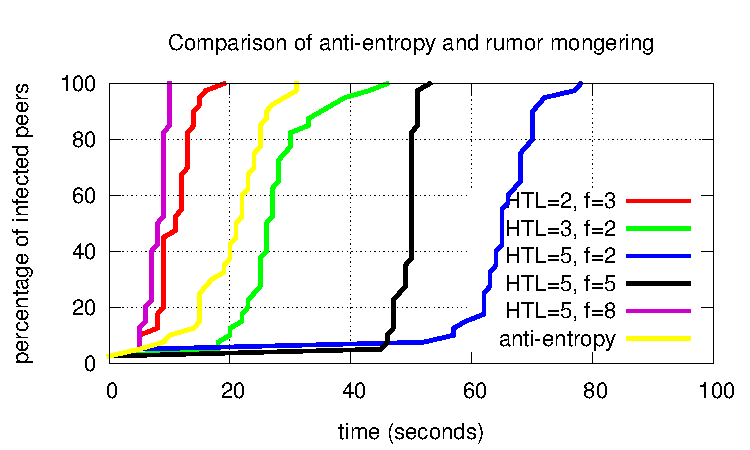
\includegraphics{rumor-mongering/plots/rm_plot_task2-2-4.pdf}
    \caption{Comparison of the anti-entropy and rumor mongering mechanims for several values of $f$ and $HTL$}
    \label{fig:task2-2-4}
  \end{figure}

  We see on this plot that as soon that $f > HTL$, the infection propagates faster with rumor mongering than
  with anti-entropy, but as soon as $f \leq HTL$ it takes more time to infect all the nodes with rumor
  mongering than with anti-entropy. We can't see a general relation between the increase of $HTL$ or $f$ and
  the increase of the propagation speed. For example, $HTL=5$ and $f=8$ is faster than $HTL=5$ and $f=2$, but
  $HTL=5$ and $f = 2$ is slower than $HTL = 3$ and $f = 2$. 

  We can also combine both protocols to run at the same time, resulting in the plot shown in Figure \ref{figure:task2.3}.

  \begin{figure}[h]
    \centering 
    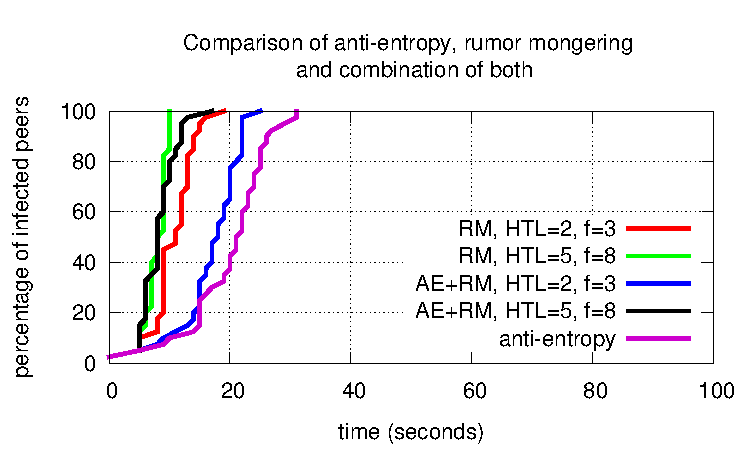
\includegraphics{rumor-mongering/rm_ae_plot_task3.pdf}
    \caption{Comparison of the anti-entropy, rumor mongering and the combination of both protocols}
    \label{figure:task2.3}
  \end{figure}

  On this example, the fastest is still rumor mongering with $HTL = 5$ and $f = 8$, although the combined
  version of rumor mongering and anti-entropy is not much slower. Both rumor mongering examples propagate
  faster than the combined version, and all propagate faster than anti-entropy alone. It is strange that the
  combined versions are not faster. Theorically, rumor mongering should seed the network at initiation
  and anti-entropy ensures that all nodes are infected. This might be due to the fact that we did not launch
  the computations in the same conditions. It is possible that for the combined version, the cluster was also
  used by other persons, resulting in slower computations, or simply we did not have luck for the random
  picks. It would certainly be more precise to launch for example 20 times the same script and then doing the
  average instead of considering just one example.
    





%%  Section 3: Peer Sampling Service
\section{Peer Sampling Service}
\label{sec:peer-sampling-service}

  In this section, we provide an implementation for the Peer Sampling Service (PSS). We used a simplified
  generic push-pull implementation. This implementation is provided in the file \texttt{pss.lua}. 
  
  We tested the PSS implementation using the three Ruby scripts provided. All the tests were run with a
  population of 50 peers, a view size of $c = 8$, $exch = 4$ and the following values of $H$ and $S$: $(H=0,
  S=0)$, $(H=0, S=4)$ and $(H=4, S=0)$.
  
  \begin{enumerate}
  \item With the \texttt{pss\_check\_partition.rb} script, we always got that the nework was connected when
    running the script.
  \item With the \texttt{pss\_check\_indegrees.rb} script, we produced the plot shown in Figure
    \ref{fig:indegrees}. The objective of the PSS is to have a gaussian distribution of indegrees around $c$,
    where $c=8$ in our case. For the Healer, we don't really see a gaussian
    distribution. We have a lot of variations (if we were to draw a tendancy curve, we would be
    tempted to take a sinusoidal one). For $H=0$ and $S=0$, it already looks a little bit more like a gaussian
    distribution, although is it not exactly centered in $c$. If we were to draw the tendancy curve of the
    Swapper, we would certainly obtain a curve similar to a gaussian, which is was the intended objective.

    \begin{figure}[h]
      \centering
      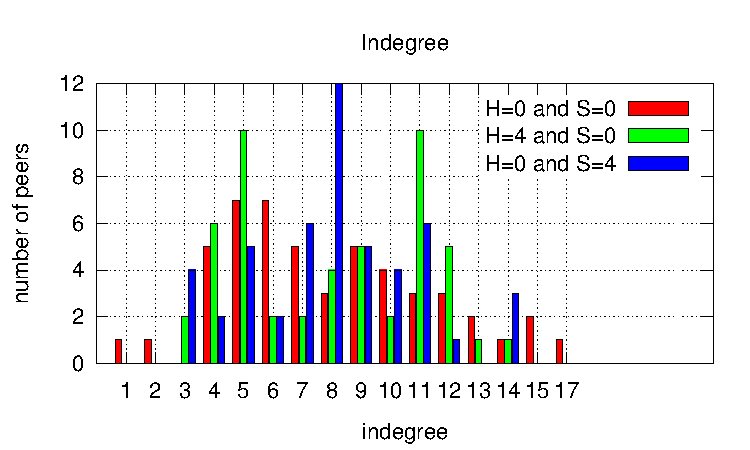
\includegraphics{"peer sampling service"/Indegree.pdf}
      \caption{Indegrees for different values of $H$ and $S$}
      \label{fig:indegrees}
    \end{figure}

  \item With the \texttt{pss\_check\_clustering.rb} script, we produced the plot shown in Figure
    \ref{fig:clustering}. We see on the plot that the clustering factor is rather similar for the three
    different choices of $H$ and $S$. The objective is to have a minimal clustering in order to maximize the
    randomness of the graph, which is best achieved with the Swapper. The clustering informally reprensents
    the fact that ``my neighbours are neighbours themselves'' (an analogy of this would be ``my facebook
    friends are friends on facebook themselves''). 


    \begin{figure}[h]
      \centering
      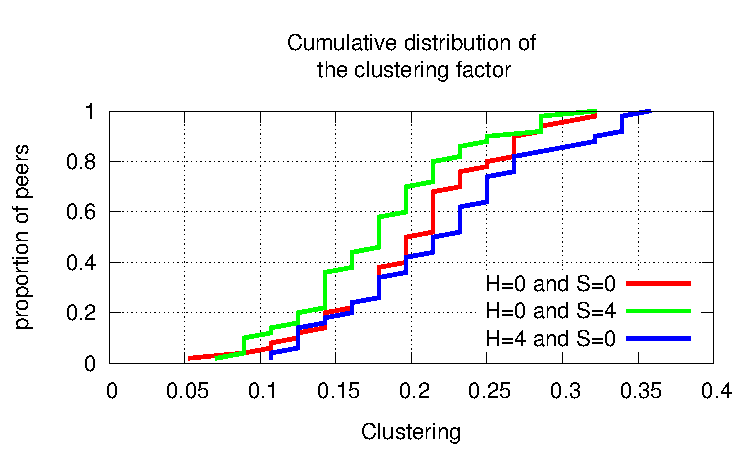
\includegraphics{"peer sampling service"/Clustering.pdf}
      \caption{Cumulative distribution of the clustering factor for different values of $H$ and $S$}
      \label{fig:clustering}
    \end{figure}

    Mathematically speaking, we can see this graph as the cumulative distribution of the density functions
    $f_1, f_2$ and $f_3$ where $f_1$ (respectively $f_2$ and $f_3$) are the probability distribution of the
    clustering factor of the PSS with $(H=0, S=0)$ (respectively with $(H=0, S=4)$ and $(H=4, S=0)$). Thus if
    we denote by $F_1$ (respectively $F_2$ and $F_3$) the cumulative distribution of $f_1$ (respectively $f_2$
    and $f_2$), we have that 
      \[F_1(a) = \int_{-\infty}^a f_1(x) dx\]
    and it represents the proportion of peers that have a clustering factor lower or equal to $a$. Based on
    this observation, we now clearly see that the Swapper is better than the two others, because we have that
      \[F_2(a) \geq F_1(a) \geq F_3(a),\]
    which means that the proportion of peers with a clustering factor lower or equal to $a$ is greater for the
    healer, then when $(H=0, S=0)$ and finally for the Healer.
  \end{enumerate}

  


%% Section 4: Plugging everything together
\section{Plugging everything together}
\label{sec:plugg-everyth-togeth}

  In this section, the objective is that anti-entropy and rumor mongering use the PSS in order to select
  their gossip partners.

  At first, we added a few boolean values like \texttt{pss\_activated} in the \texttt{gossip\_pss.lua} script
  (which is based on the combined anti-entropy and rumor mongering script) and then required the
  \texttt{pss.lua} script as a module. These booleans permit to choose whether to use the PSS, anti-entropy
  and rumor mongering or not. We just had to comment a few lines in \texttt{pss.lua} and it worked
  quite well, but it was not practical to launch it on the cluster. So we basically made a new file
  \texttt{gossip\_pss\_web.lua} which was the concatenation (plus or minus a few details) of the two previous mentionned
  files. We directly implemented a \texttt{getPeers(n)} function that returns $n$ peers (it is more practical
  for the rumor mongering mechanism).

  With this script, we could produce the plot in Figure \ref{fig:pss_delay}. We let the PSS run 60 seconds
  before launching the anti-entropy and rumor mongering mechanisms.

  \begin{figure}[h]
    \centering
    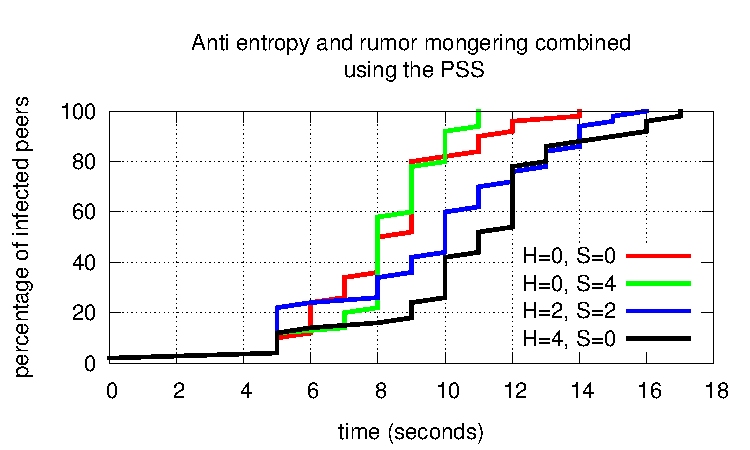
\includegraphics{"peer sampling service"/Gossip_pss.pdf}
    \caption{Delay of reception of one message using the PSS with various values of $H$ and $S$ and the
      combined version of the anti-entropy and rumor mongering mechanisms.}
    \label{fig:pss_delay}
  \end{figure}

  We actually see that the Swapper is the best. But with what we explained in section
  \ref{sec:peer-sampling-service}, it is not surprising. It had the best indegrees and clustering
  properties. The fact that the clustering factor is low implies that there are not too much redundant
  messages with anti-entropy, and there are more chances to choose a peer owning a new message with
  anti-entropy. 

  If we compare Figure \ref{fig:pss_delay} with Figure \ref{figure:task2.3}, we see that on the former, the
  nodes are infected faster (we used a population of 50 peers for the PSS and a population of 40 peers for
  task 2.3). Although it is hard to compare both plots further as the parameters are not the same, we can see
  that the PSS helps the propagation, because the resulting graph has good properties.

%% Section 5: Conclusion
\section{Conclusion}
\label{sec:conclusion}

  
  The first part of the project was consecrated to the implementation of two gossip-based dissemination
  protocols, namely anti-entropy and rumor mongering. We evaluated their performances in terms of delay when
  they were used separately or at the same time. We found that depending on the values of $f$ and $HTL$, 
  anti-entropy was more efficient than rumor mongering. Still depending on the values of $f$ and $HTL$, the
  combination of both mechanisms was faster than rumor mongering and anti-entropy. In this part, we made the
  unrealistic assumption that each node in the system has a global view of the network.

  This lead us to the second part of the project, namely implementing the Peer Sampling Service. We had to
  test the properties of the graph produced by the PSS:
  \begin{itemize}
  \item is the network connected?
  \item how clustered is it?
  \item what is the indegrees of the nodes?
  \end{itemize}
  We found out that the Swapper protocols ($H=0$ and $S=4$) had the best properties, the cluster factor was
  lower and the indegree distribution was similar to a gaussian distribution centered at $c$.

  Eventually, we could use our implementation of the PSS to ameliorate the gossip-based dissemination
  protocols seen in the first part. The observation was that the PSS helped the dissemination because of the
  graph's good properties.












	
\end{document}



%%% Local Variables:
%%% mode: latex
%%% TeX-master: t 
%%% End: